\chapter{Simulação}

Para verificar o funcionamento do sistema nas vias, foram realizadas simulações, em computador, de situações com diferentes modos de funcionamento. Com os resultados obtidos, foi possível reconhecer o impacto que o sistema teve no fluxo veicular, de acordo com a abordagem escolhida.

Foi escolhido um ambiente de simulação onde é possível construiur cenários, com os parâmetros desejados, e fazer comparações entre diferentes situações envolvendo o semáforo.
O software utilizado para realizar a simulação foi o SUMO (Simulation of Urban MObility), em conjunto com o módulo para python, TraCI (Traffic Control Interface).
%[http://www.planalto.gov.br/ccivil_03/LEIS/L9503.htm]

\section{SUMO}
%http://www.sumo.dlr.de/pdf/sysmea_v5_n34_2012_4.pdf
% "Recent Development and Applications of SUMO - Simulation of Urban MObility"; Daniel Krajzewicz, Jakob Erdmann, Michael Behrisch, and Laura Bieker. International Journal On Advances in Systems and Measurements, 5 (3&4):128-138, December 2012.
SUMO é um pacote de simulação de tráfego, com capacidade de gerar cenários de proporções variadas, de pequenos trechos a cidades inteiras. O projeto foi iniciado em 2001, pelo Institute of Transportation System, no German Aerospace Center, e foi feito público em 2002, mantendo até os dias atuais, a condição de projeto open source.
O software foi criado com o intuito de prover uma ferramenta para auxiliar pesquisas relacionadas a tráfego urbano de veículos e pedestres\cite{sumo}. 
  
\subsection{TraCI}  

TraCI (Traffic Control Interface) é uma ferramenta que permite ao usuário ter acesso às simulações, realizadas pelo SUMO, enquanto elas acontecem. É possível adquirir valores de elementos simulados, como semáforos e detectores.
Para obter acesso ao SUMO, a ferramenta utiliza uma arquitetura baseada em comunicação TCP entre cliente e servidor, com o SUMO agindo como servidor e o TraCI acessa os dados e envia comandos como o cliente\cite{sumo}.

Essa ferramenta é utilizada por meio de um módulo, que apresenta funções que podem ser utilizados para adquirir dados e enviar comandos para a simulação. Para esse projeto, o módulo foi utilizado em um script, escrito na linguagem de programação Python, em que os comandos foram utilizados, juntamente com uma lógica para realizar o controle semafórico, para monitorar os semáforos e os detectores veiculares.

\subsection{Cenários}

O software permite ao usuário bastante controle sobre a criação dos cenários a serem simulados. Antes de iniciar uma simulação, é necessário criar a estrutura física que delimita os caminhos possíveis, que seriam as vias. Para isso, o usuário deve criar pontos de referência, ou nodes, que são utilizados como origem e/ou destino. Esses nodes são ligados entre si por elementos chamados edges, que representam as vias, por onde os veículos passarão. Ao definir as edges, além de escolher quais nodes serão ligados, é definido também o sentido da via (definindo qual node é origem, e qual é destino). É nessa etapa onde são definidos os nodes que terão semáforos.

Após a criação da estrutura, é necessário definir o comportamento dos elementos que participarão da simulação. Tal comportamento é definido por meio de parâmetros, nos arquivos de configuração do SUMO.

\subsection{Configurações}

Com a estrutura criada, a próxima etapa é definir as configurações dos veículos, dos detectores, se forem utilizados, e dos semáforos. O software permite a separação de veículos em diferentes tipos, cada um com valores de velocidade, caminhos a percorrer e tempo de entrada na simulação. Além disso, é possível criar fluxos de carro, que geram carros com os mesmos parâmetros, sem ser necessária a criação de cada veículo, separadamente, nos arquivos de configuração.

Nas configurações referentes aos semáforos, é possível estabelecer planos semafóricos a serem seguidos. Planos são uma representação do estado de acendimento de um semáforo (quais cores serão acesas em quais caminhos), com um parâmetro de tempo de duração. Ao utilizar o TraCI, é possível realizar a troca de planos de um semáforo em tempo real, sem precisar alterar os arquivos de configuração.

Os detectores são declarados em um arquivo de configuração, onde são definidos em qual rota serão posicionados, e em que ponto dessa rota, assim como o intervalo de tempo entre uma detecção e outra. Os detectores são elementos que podem ser monitorados pelo script criado para rodar o TraCI, possibilitando adicionar uma camada de dinamismo à simulação.

\subsection{Aquisição de dados}

O software permite a exportação de arquivos com diferentes tipos de dados, referentes aos veículos, aos caminhos e aos detectores. A exportação desses arquivos deve ser definida no momento da configuração da simulação, o que gera um arquivo separado, para cada parâmetro desejado, no formato xml. Os dados exportados são obtidos a cada passo da simulação e apresentados na ordem de aquisição.

Ao usar o TraCI, porém, é possível realizar o monitoramento de parâmetros em tempo real. Pode-se monitorar o padrão de acendimento de um semáforo, por exemplo, e de acordo com a lógica do programa, modificar o estado do mesmo como desejado. O TraCI permite realizar a leitura de detectores, atuando como laços indutivos, na pista, obtendo-se dados referentes à contagem de veículos em um determinado caminho, assim como velocidade da via.

\subsection{Testes realizados}

Para realizar os testes, foi criado, utilizando o software SUMO, um ambiente de simulação composto por um cruzamento, simples, como pode ser visto na figura \ref{simulationLayout}, com quatro possíveis caminhos a serem percorridos pelos veículos. Os caminhos disponíveis são iniciados nos nodes 1, 2, 3 e 4, e finalizados nos nodes 3, 4, 1 e 2, respectivamente. 
Todos os caminhos passam pelo node 0, no centro da simulação, onde se encontra o semáforo. Essa mesma estrutura foi utilizada nas quatro simulações realizadas.

\begin{figure}[ht]
    \begin{center}
    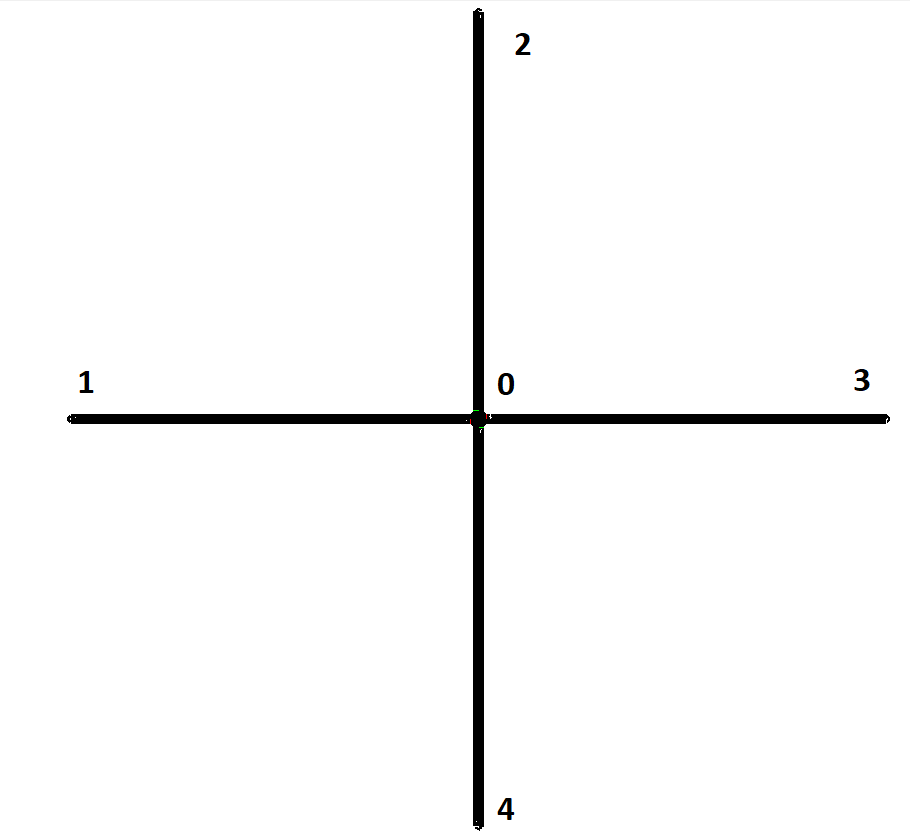
\includegraphics[width=0.5\textwidth]{figuras/Simulation_Scenario.png}
    \end{center}
    \caption[Estrutura da simulação]{\textit{Layout} do cruzamento e numeração dos \textit{nodes}.}
    \label{simulationLayout}
\end{figure}

%Car-following krauss model https://elib.dlr.de/115720/1/esm_bieker.pdf
Além da estrutura da via, a mesma configuração foi utilizada para os veículos que trafegaram pelos quatro caminhos, em todas as simulações. Para gerar os veículos, foram criados quatro fluxos, um para cada caminhos, que emitiam carros com as mesmas propriedades. A emissão de veículos, nesse software, obedece a uma distribuição binomial, onde a cada passo da simulação, existe uma probabilidade de um veículo ser emitido à via. Além disso, o simulador adota o modelo de car-following de Krauss, que rege o comportamento de cada veículo, quando há outros veículos a sua frente\cite{krauss}.

As configurações utilizadas para a criação do semáforo foi um plano composto de dois estados. No primeiro estado, o semáforo fica verde para os caminhos partindo dos nodes 1 e 3 em direção aos nodes 3 e 1, respectivamente, e fica vermelho para os outros dois caminhos. No segundo estado, os acendimentos se invertem, permitindo a passagem dos caminhos originados nos nodes 2 e 4. Cada estado tem uma duração de trinta segundos, com uma transição de três segundos, para os focos verdes passarem para amarelo e depois vermelho.

\begin{figure}[ht]
    \begin{center}
    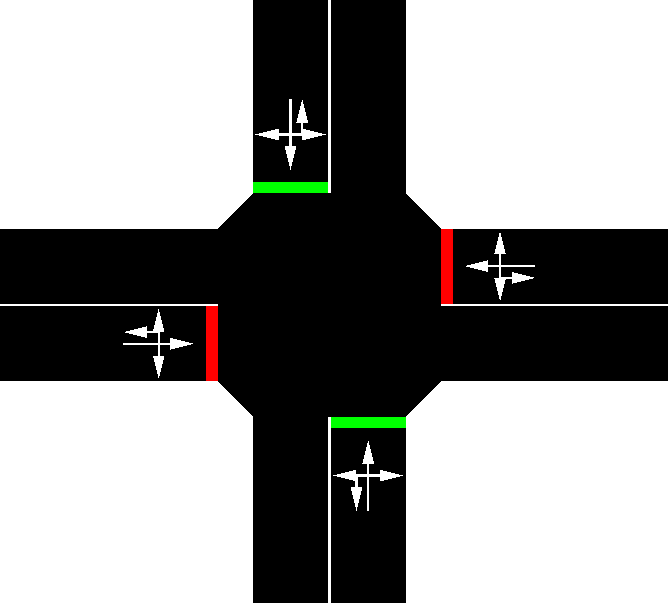
\includegraphics[width=0.4\textwidth]{figuras/Traffic_Light.PNG}
    \end{center}
    \caption[Semáforo simulado]{Semáforos localizados no \textit{node} zero.}
    \label{TrafficLight}
\end{figure}

Para executar as simulações, foi escrito um escrito, em python, que age como o controlador da simulação. Esse script executa o programa, utilizando os arquivos de configuração, determina quando os passos da simulação serão dados e monitora os elementos em tempo real. Esse script utiliza o módulo do TraCI para realizar suas funções.

No primeiro teste, foi realizada uma simulação sem o sistema em funcionamento (cruzamento sem semáforos).

No segundo teste, o sistema foi implementado no cruzamento, utilizando planos de tempo fixo, em que cada estado do semáforo está pré-definido e não há alteração de tempos ou ordem de abertura.

No terceiro teste, o sistema passou a funcionar no modo adaptativo, contando com um detector, agindo como um laço indutivo, colocado na via, que envia dados em tempo real para o controlador da simulação, sendo assim possível realizar um sistema que se adapte, enquanto o programa está rodando. O detector, como pode ser visto na figura \ref{simulationThree}, foi instalado no caminho que parte do node 2 e segue para o node 4.
Nesse teste, o controle dos tempos foi realizado por demanda (pela quantidade de carros esperando no semáforo fechado).

\begin{figure}[ht]
    \begin{center}
    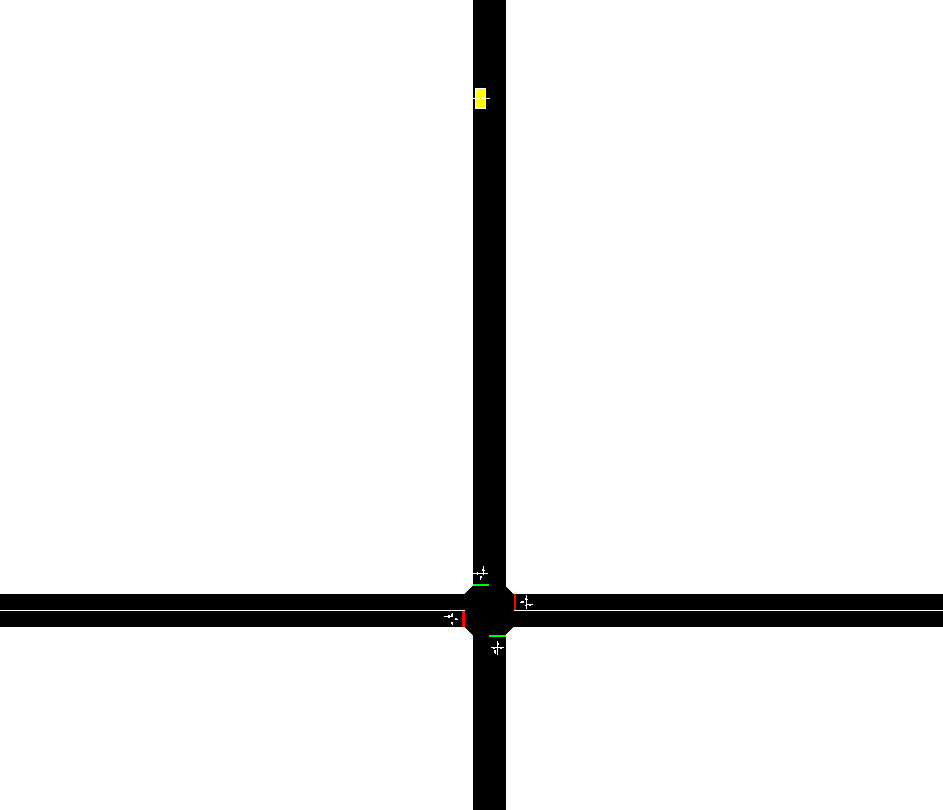
\includegraphics[width=0.4\textwidth]{figuras/Simulation_3_Zoom.PNG}
    \end{center}
    \caption[Simulação com um detector veicular]{Detector utilizado para modo adaptativo.}
    \label{simulationThree}
\end{figure}

No quarto teste, foram utilizados dois detectores, como pode ser visto na figura \ref{simulationFour}, um no caminho que parte do node 2 e parte para o node 4, e outro no caminho que parte do node 3 e parte para o node 1. Nessa simulação, o semáforo funcionou com os dois estados com tempo variável. Cada detector representa um elemento monitorado pelo script que controla a simulação. 

uma característica importante do modo adaptativo é que existe um limite de tempo máximo que o semáforo pode permanecer em um estado. Isso evita situações em que o semáforo fique preso em um único estado.

Todos os testes foram realizados sob as mesmas configurações de via e de emissão de veículos, tendo como diferença apenas o modo em que o semáforo funcionou (ou, no primeiro caso, a ausência do mesmo). Assim, pode-se facilmente observar o impacto que o sistema teve em cada cenário.

\begin{figure}[ht]
    \begin{center}
    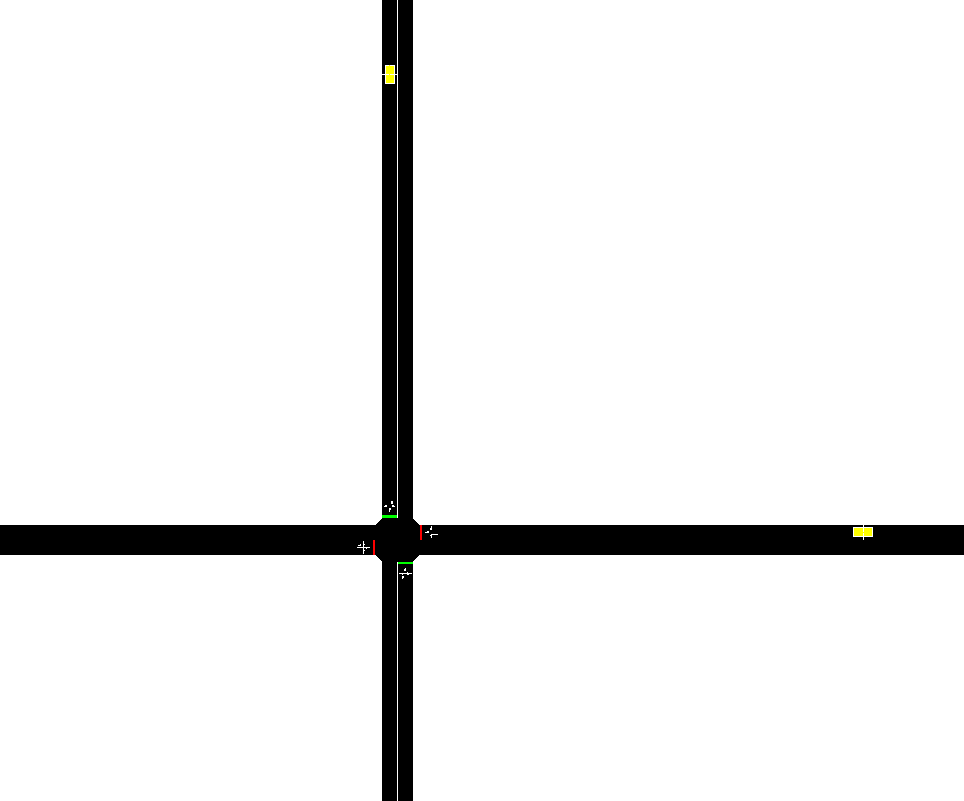
\includegraphics[width=0.4\textwidth]{figuras/Simulation_4_Zoom.PNG}
    \end{center}
    \caption[Simulação com dois detectores veicular]{Simulação com dois detectores.}
    \label{simulationFour}
\end{figure}